\chapter{System Methodology and Design}
\section{General Description}
As the product of this final project, an application named TELUR IRIS (Telkom University Indoor Routing System) was made. This application is used for finding the shortest path between two rooms of Telkom University. Although, as declared in scope section of Chapter I, this application still use the data of D, E, and F Buildengs only. This application will show the user clearly about how the nodes of the graph represent the buildings by showing the nodes based on its three dimensional attribute. Several kinds of shortest path algorithm will be implemented and will be analyzed to get algorithm wich will give the best prformance that match this case.
  
\section{System Design}

\subsection{The Data Structure}
Dataset that used in this final project is the spatial data of Faculty of Informatics Telkom University, Bandung that include D, E, and F buildings. Figure \ref{fig:figure13} is the table relation of the dataset used in the TELUR IRIS Application. We need the data of buildings, rooms, corridors, stairs, and also Segments wich will be the relation or edges in the graph. For rooms, corridors, and stairs will have an attribute Building\textunderscore{ID} as a foreign key that reference to Building\textunderscore{ID} as the primary key of buildings. With this way, we know that each of rooms, corridors, and stairs is belongs to one of the buildings. However, for the corridor nodes that are outside the buildings, the Building\textunderscore{ID} attribute will be set as null value. Segments table has source and destination attribute that actually filled with the nodes ID in graph. 

\vspace{60mm}

\begin{figure}[h!]
	\centering
	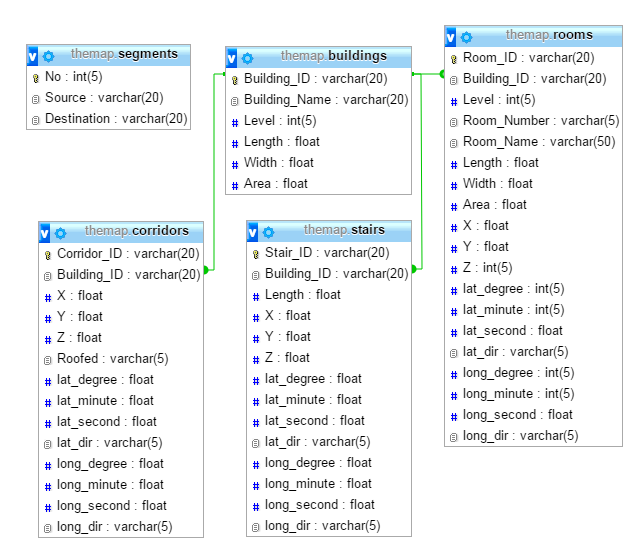
\includegraphics[scale=0.9]{figure13.png}
	\caption{Relational table of dataset}
	\label{fig:figure13}
\end{figure}

\vspace{60mm}

\subsection{System Flow}
The main process of this application can be modeled with the flow chart below.

\begin{figure}[h!]
	\centering
	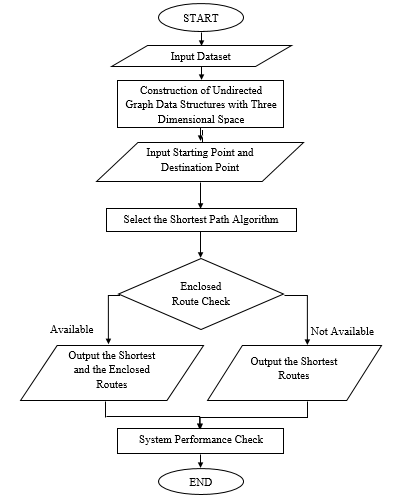
\includegraphics[scale=1.4]{figure14.png}
	\caption{System Flow Chart}
	\label{fig:figure14}
\end{figure}

\subsubsection{Construction of undirected Graph Data Structures with Three Dimensional Space}
At this stage, the construction of undirected graph data structure using three dimensional space representation of the existing data sets. Unlike the indoor routing data representation that already described in Chapter 2, this will represent multi-floor building in three dimensions based on the location of the coordinates x, y, and z coordinates of altitude. This final project use the study case of D, E, and F buildings of School of Computing in Telkom University, Bandung, Indonesia. Figure \ref{fig:figure19a} shows the area of Telokm University captured from Google Earth Application. The red rectanges are the D, E, and F buildings. Figure \ref{fig:figure19b}shows the zoomed in figure of D, E, and F buildings with the 2D graph modeling overlayed it. This is a way to get the longitude and latitude coordinates. 

\begin{figure}[h!]
	\centering
	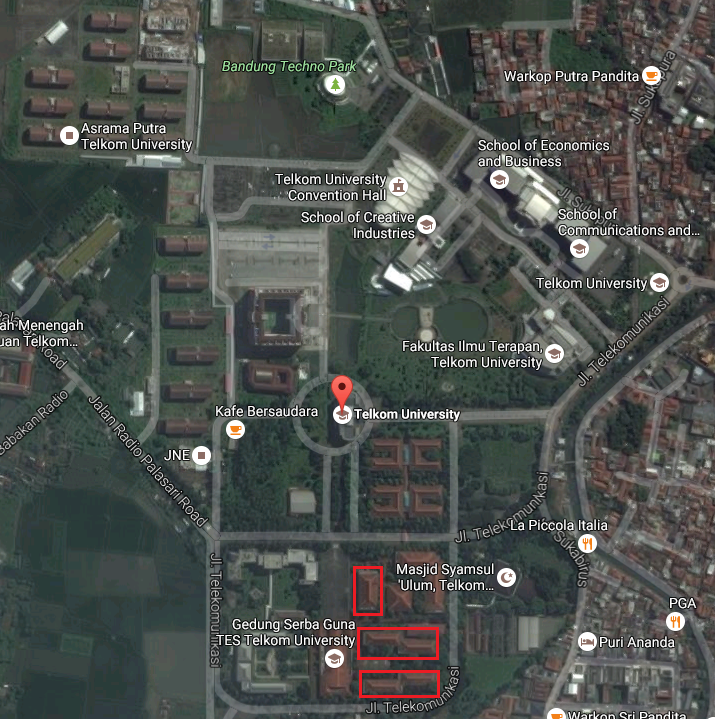
\includegraphics[scale=0.7]{figure19a.png}
	\caption{Telkom University area}
	\label{fig:figure19a}
\end{figure}

\begin{figure}[h!]
	\centering
	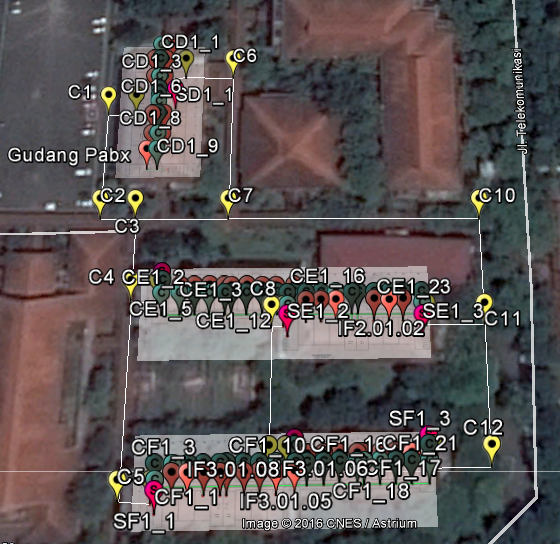
\includegraphics[scale=1]{figure19b.png}
	\caption{Telkom University area}
	\label{fig:figure19b}
\end{figure}



In the next step, the 3D modelling can be implemented in the system. This system show the 3D model as 2D model like shown in Figure \ref{fig:figure18} because a building is actually an overlayed multi-objects. To show the 3D modelling, coordinate shifting method could be implemented. Coordinate shifting method will move the x and y coordinate of the nodes so it would not be overlayed anymore. Illustration of Three Dimensional Spaces model can be seen in Figure \ref{fig:figure15}. red nodes mean the first level, green nodes mean the second floor, and blue ones mean the third floor.

\begin{figure}[h!]
	\centering
	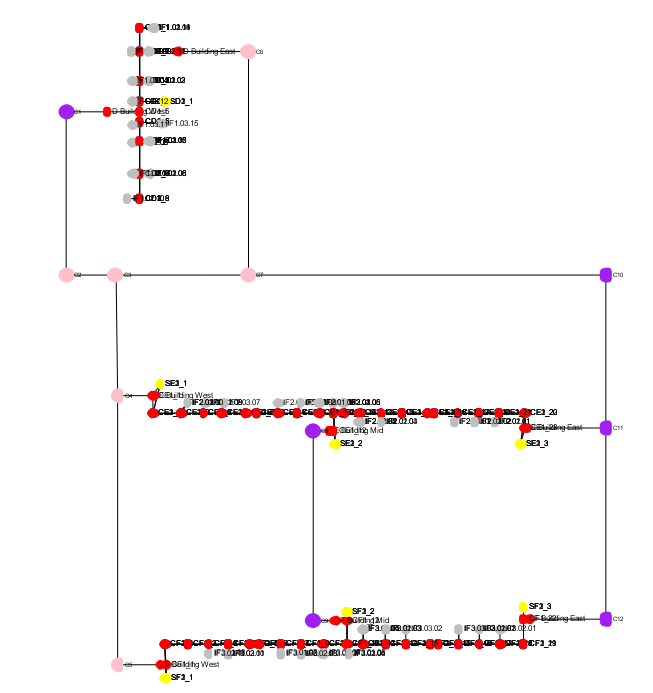
\includegraphics[scale=0.5]{figure18.PNG}
	\caption{2D system's graph modeling}
	\label{fig:figure18}
\end{figure}

\begin{figure}[h!]
	\centering
	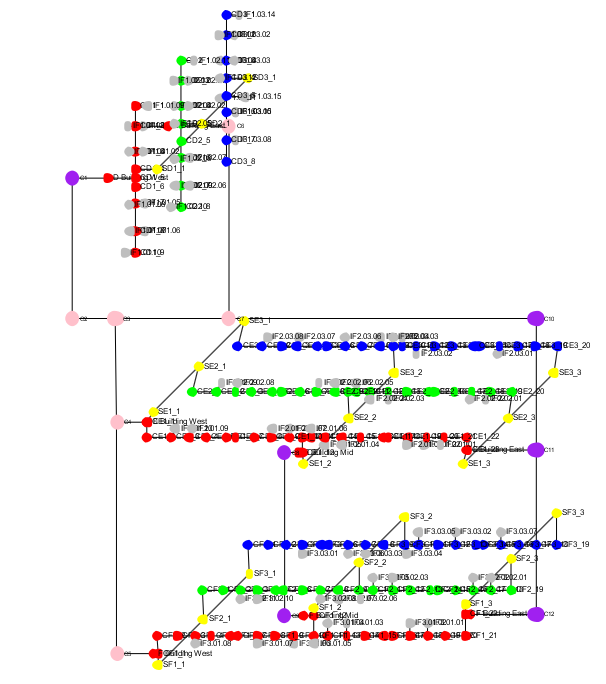
\includegraphics[scale=0.5]{figure15.PNG}
	\caption{3D system's graph modeling}
	\label{fig:figure15}
\end{figure}

\vspace{10mm}
\subsubsection{Finding the Shortest Path}
At this stage, shortest path algorithms will be implemented. There are Dijkstra's, Bellman-Ford, Floyd-Warshall, and A* algorithms that we could try to give the result of the shortest path. After the user choose one of the algorithms, shortest path searching will be done twice. The first search is using the full part of graph to show the shortest path weather it is open or close path. The second search will be eliminate nodes wich are the open space, so it will return a closed path.

By default, the system will show the close space path like the one shown in Figure \ref{fig:figure16}. But, by clicking the shortest path text area, it could easily change the view to the shortest path like shown in Figure \ref{fig:figure17}.

\begin{figure}[h!]
	\centering
	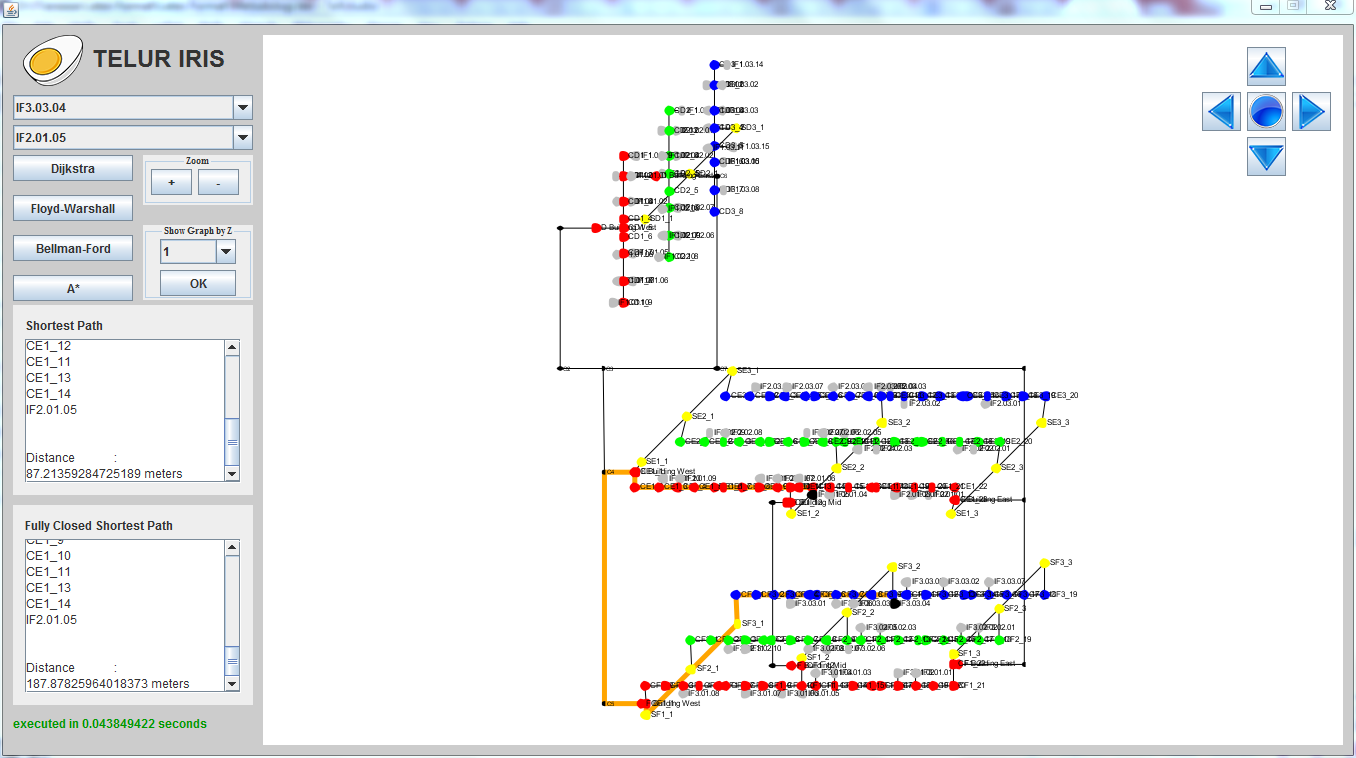
\includegraphics[scale=0.4]{figure16.PNG}
	\caption{The close space shortest path}
	\label{fig:figure16}
\end{figure}

\begin{figure}[h!]
	\centering
	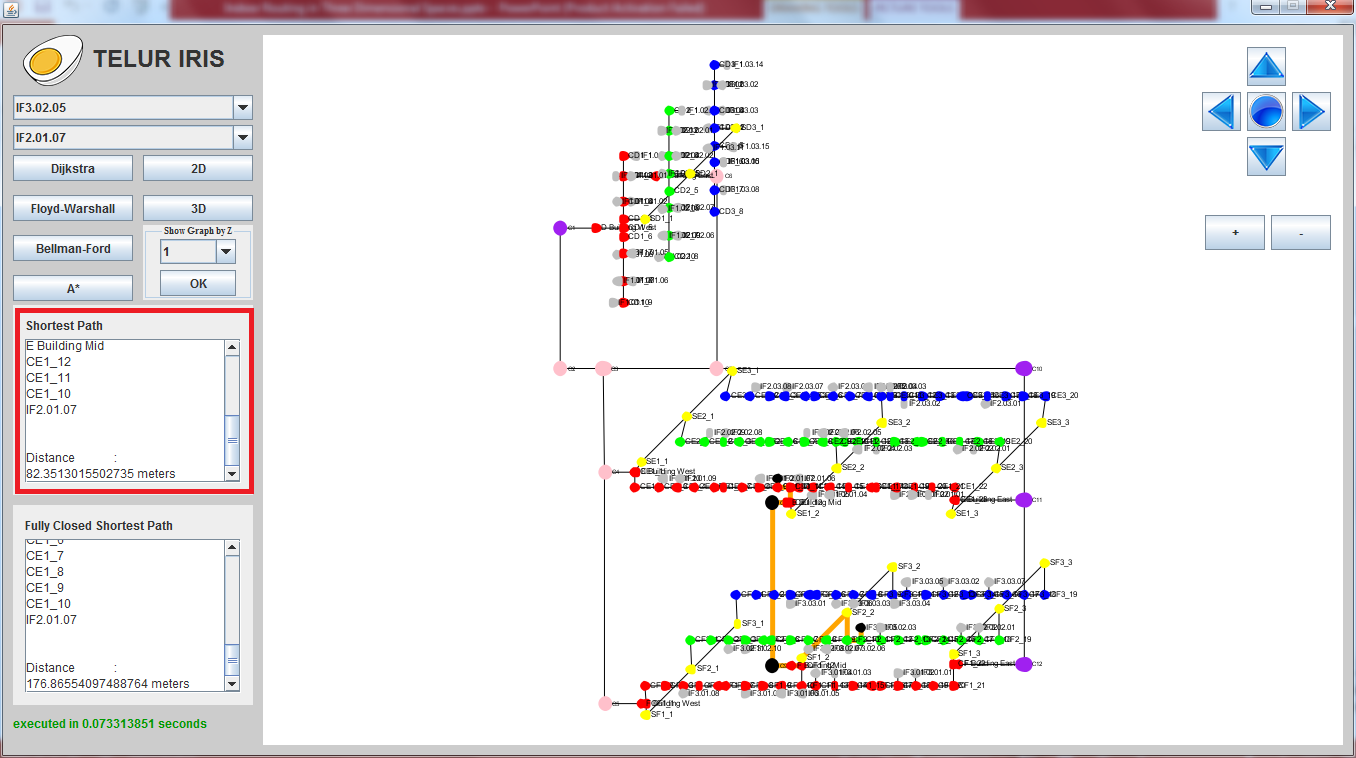
\includegraphics[scale=0.4]{figure17.PNG}
	\caption{The shortest path}
	\label{fig:figure17}
\end{figure}

\vspace{60mm}
\subsubsection{System Performance Check}
After the algorithm return the shortest paths, time execution will be measured at this stage.

\section{System Requirements Specification}
In this final project, the hardware and software that will support routing indoor systems to be built and work properly are:

\begin{enumerate}
	\item Hardware Specification\\
		Here is the following hardware specifications used in this final project.\\
		Model 	: Intel® Core™ i7-3770 CPU\\
		Prosesor	: 3.40 GHz Intel Core i7\\
		RAM	: 4 GB\\
		OS		: Windows 7 Professional 64 bit

	\item Software Specification\\
Here is the following software specifications used in this final project.\\
Application	:
\begin{itemize}
	\item Java Netbeans IDE 8.0.2
	\item JDK 1.8
	\item MySQL
\end{itemize}
\end{enumerate}

\section{Summary}
This chapter is about the plan of how to construct the Indoor Routing System using three dimensional spaces data structure. It also axplain the detail of the system flow and the system requirements.